% REMEMBER: You must not plagiarise anything in your report. Be extremely careful.
\documentclass{l4proj}
\usepackage{dirtytalk}
\usepackage{caption}
\usepackage{subcaption}
\usepackage{tikz}
\usepackage{float}

\usetikzlibrary{shapes,arrows}

\tikzstyle{decision} = [diamond, draw, fill=blue!20, 
    text width=4.5em, text badly centered, node distance=3cm, inner sep=0pt]
\tikzstyle{block} = [rectangle, draw, fill=blue!20, 
    text width=5em, text centered, rounded corners, minimum height=4em]
\tikzstyle{line} = [draw, -latex']
\tikzstyle{cloud} = [draw, ellipse,fill=red!20, node distance=3cm,
    minimum height=2em]
    

\begin{document}

%==============================================================================
%% METADATA
\title{Lipid Kinetics Inference Software}
\author{Marc William Elrick}
\date{\today}
\maketitle

%==============================================================================
%% ABSTRACT
\begin{abstract}

    
    The inference of lipid kinetics is a useful tool for understanding how metabolic reactions work within different biological organisms. This dissertation discusses the development of Lipid Kinetics Inference Software, an application for performing such inference that is a dramatic improvement over the previous state of the art. It provides an introduction to the problem at hand before discussing the entire software development life-cycle including: requirements gathering; design; implementation; software engineering and DevOps practices; and usability evaluation. It then gives reflections on this process and lists suggestions for future work. Evaluations showed that while the application was effective in performing analysis, there were several usability issues that were later remedied.
\end{abstract}

%==============================================================================

% EDUCATION REUSE CONSENT FORM
% If you consent to your project being shown to future students for educational purposes
% then insert your name and the date below to  sign the education use form that appears in the front of the document. 
% You must explicitly give consent if you wish to do so.
% If you sign, your project may be included in the Hall of Fame if it scores particularly highly.
%
% Please note that you are under no obligation to sign
% this declaration, but doing so would help future students.
%
\def\consentname {Marc Elrick} % your full name
\def\consentdate {\today} % the date you agree
%
\educationalconsent


%==============================================================================
\tableofcontents

%==============================================================================
%% Notes on formatting
%==============================================================================
% The first page, abstract and table of contents are numbered using Roman numerals and are not
% included in the page count. 
%
% From now on pages are numbered
% using Arabic numerals. Therefore, immediately after the first call to \chapter we need the call
% \pagenumbering{arabic} and this should be called once only in the document. 
%
% Do not alter the bibliography style.
%
% The first Chapter should then be on page 1. You are allowed 40 pages for a 40 credit project and 30 pages for a 
% 20 credit report. This includes everything numbered in Arabic numerals (excluding front matter) up
% to but excluding the appendices and bibliography.
%
% You must not alter text size (it is currently 10pt) or alter margins or spacing.
%
%
%==================================================================================================================================
%
% IMPORTANT
% The chapter headings here are **suggestions**. You don't have to follow this model if
% it doesn't fit your project. Every project should have an introduction and conclusion,
% however. 
%
%==================================================================================================================================
\chapter{Introduction}

% reset page numbering. Don't remove this!
\pagenumbering{arabic} 


This chapter provides an introduction to the LiKInS(Lipid Kinetics Inference Software) application and the motivations behind its development. It gives a cursory description to the process of isotope labelling within the context of lipidomics before discussing the project aims and the clients involved. The chapter concludes with an outline of the rest of this dissertation. While this chapter provides a cursory description of the problem being solved, chapter \ref{background} provides a much more in-depth explanation.

\section{Problem Description} \label{problem-description}
In order to grasp the problem being solved by LiKInS, it is first necessary to gain a basic understanding of where the data being processed originates. The following subsections each discuss topics necessary to understand the bigger picture. 

\subsection{Isotopes \& Isotope Labelling}
An isotope is defined by \cite{isotope} as \say{one of two or more species of atoms of a chemical element with the same atomic number and position in the periodic table and nearly identical chemical behaviour but with different atomic masses and physical properties.} Isotopes are essentially all of the variants of an element, each of which has a differing number of neutrons.

Isotope labelling is an experimental technique used in various scientific fields to observe and measure the effects and activity of a chemical reaction. A reactant (the substance undergoing the reaction) is deliberately altered by replacing some of its atoms with a less common isotope (an atom of the same element with a differing number of neutrons). Researchers then allow the reaction to take place and, after time has passed, they can examine the products to measure how much of the isotope is present, allowing them to determine the sequence of events within the reaction. 

\subsection{Lipids \& Lipidomics}
Lipids are defined by \cite{lipidDef19:online} as being \say{any of a diverse group of organic compounds including fats, oils, hormones, and certain components of membranes that are grouped together because they do not interact appreciably with water.} For the purposes of this dissertation, they can be thought of as simply interesting organic molecules that can be produced in metabolic reactions.

Metabolomics  is defined as \say{the study of metabolites, the chemical substances produced as a result of metabolism, which encompasses all the chemical reactions that take place within cells to provide energy for vital processes} \citep{Metabolomics}. Lipidomics is a sub-branch of metabolomics concerned specifically with the pathways of lipids within biological systems and how they interact with other metabolites. Isotope labelling can be used to observe and improve our understanding of these pathways. This project deals specifically with the analysis of isotope labelling data within lipidomics.

\subsection{Mass Spectrometry \& LiKInS}
The measurement of products is done using an experimental technique known as mass spectrometry via a piece of specialised hardware known as a mass-spectrometer. The resulting data is stored as a MZML file. All files utilised during the development of LiKInS were created using measurements from an Orbitrap Exactive mass-spectrometer \citep{thermofisher}. Prior to the development of LiKInS, there was no publicly available software for analysing how the intensity of isotopes within products vary across time-points within a reaction. LiKInS allows the user to specify a set of lipids and a set of experiment files before parsing and analysing these files to produce an excel spreadsheet with the analysed data and accompanying visualisations.



\section{Clients}\label{clients}
LiKInS was developed in collaboration with metabolomics researchers from both the University of the Highlands and Islands and Glasgow Polyomics. These clients provided much of the background information for the project and served as the target users for the software. Towards the latter stages of development, they provided feedback and assisted in the gathering of new requirements and improvements to the application. They also acted as particpants for the usability evaluation and assisted in recruiting other participants. 

\section{Motivations}
The analysis process performed by LiKInS could previously only be done manually unless the researcher had a significant amount of programming experience. As is discussed in-depth in section \ref{manual-process}, the manual processing of this data is incredibly time consuming and requires the large-scale inspection and copying of values and so leaves a high potential for human error. The motivation is therefore clear: by developing an application to allow the automation of this process, researchers can save hours of tedious and laborious work. 

This stated motivation was validated at the end of the project when one of the clients, who had previously undertaken the manual analysis process, gave the following statement via email: \say{The process isn’t ridiculously difficult however because it is not very automatic it takes up a fair amount of time. If this was reduced I could have monitored more lipids for my PhD}. It is clear that the concept of LiKInS has clear scope to increase the velocity of research within this area.

\section{Aims}
Given the problem description provided in \ref{problem-description}, the main objective of this project was clear: to develop an open-source application that can parse and analyse MZML files to produce output data and visualisations stored as a spreadsheet. A prototype analysis pipeline was provided as a Jupyter notebook so in essence, the aim was to turn this into a self-contained, user-focused desktop application. This is discussed further in chapter \ref{requirements-gathering}, while the entire development process for this software is the subject matter of this dissertation.


\section{Dissertation Structure}
This dissertation will outline the design, implementation and evaluation of LiKInS, as well as the software engineering practices utilised throughout. The remaining chapters are as follows:
\begin{itemize}
    \item \textbf{Chapter 2 - Background}\newline
    This chapter gives a more in-depth problem description and introduces the concepts and experimental processes that lead to the conceptualisation of LiKInS. It also reports on the previous state of the art in inferring lipid kinetics as well as previous work that contributed to the creation of LiKInS.
    \item \textbf{Chapter 3 - Requirements Gathering}\newline
    This chapter is concerned with the process of gathering requirements, including how the problem was first understood, the development of user stories, functional and non-functional requirements and how new requirements were gathered during implementation and evaluation.
    \item \textbf{Chapter 4 - Design}\newline
    Chapter 4 covers the design process of the software, including the user interface design, the system architecture design and refinements to the design during development.
    \item \textbf{Chapter 5 - Implementation}\newline
    This chapter discusses the implementation of LiKInS, including the technology stack, GUI development, state management system, packaging and testing
    .
    \item \textbf{Chapter 6 - Software Engineering Practices}\newline
    This chapter discusses the software engineering and DevOps practices that were utilised, including version control, issue tracking, wiki documentation, continuous integration, deployment and test-driven development. 
    \item \textbf{Chapter 7 - Usability Evaluation}\newline
    Chapter 7 discusses how the usability of the software was evaluated. This includes the recruitment of participants, the protocol used and how gathered data was analysed.
    \item \textbf{Chapter 8 - Conclusion}\newline
    The final chapter provides a summary of and reflections on the development of LiKInS as well as thoughts on future improvements that could be made.
    
\end{itemize}


%==================================================================================================================================
\chapter{Background}\label{background}
This chapter discusses key concepts behind the analysis process as well as the previous state of the art for inferring lipid kinetics. I then goes on to discuss previous contributions and how they lead to the development of LiKInS.


\section{In-Depth Problem Description}
With the relevant definitions being provided in section \ref{problem-description}, it is now possible to give a more specific description of the analysis process and the surrounding experimental process.

\subsection{Heavy-Water}
Much of this chapter will use the example of heavy water to explain the isotope labelling process. It is therefore important to understand how heavy-water differs from ordinary water. Whilst the vast majority of water molecules have chemical formula $H_{2}O$, where $H$ is hydrogen-1, also known as protium (the most abundant hydrogen isotope with one proton and no neutrons), heavy-water molecules have chemical formula $D_2O$ (also written as $^{2}H_{2}O$), where $D$ is deuterium. Deuterium, or hydrogen-2, is an isotope of hydrogen which has one proton and one neutron. The difference between these isotopes is illustrated in figure \ref{fig:h1-vs-h2}.
%References for distribution of H to D%
If one were to take a sample of water from a naturally occurring source (e.g. the ocean), that sample would contain approximately 1 deuterium atom for every 6,700 \citep{heavy-water} protium atoms. This means that while $H_{2}O$ does occur naturally, it is extremely rare. Henceforth, \say{ordinary water} refers specifically to $H_2O$.


\begin{figure}[htb]
\centering
\begin{subfigure}{0.3\linewidth}
        \includegraphics[width=\linewidth]{dissertation/images/Hydrogen-1.pdf}
        \caption{Hydrogen-1 (Protium) Atom}
    \end{subfigure}
    \begin{subfigure}{0.3\linewidth}
        \includegraphics[width=\linewidth]{dissertation/images/Deutereum.pdf}
    \caption{Hydrogen-2 (Deuterium) Atom}
    \end{subfigure}
    \caption{Diagram showing the difference between protium and deuterium atoms. While the nucleus of a protium atom contains one proton and no neutrons, the nucleus of a deuterium atom contains one proton and one neutron.}
    \label{fig:h1-vs-h2}
\end{figure}

\subsection{Definitions}
Four terms that are relevant to this problem description are as defined. \textbf{Mass-charge ratio}, or m/z, is the ratio of atomic mass to formal charge of an ion (a charged particle, in our case a lipid). \textbf{Adducts} are molecules that are formed via the addition of two separate molecules. \textbf{Retention time} is the time from a sample being entered into the mass-spectrometer to becoming visible on its chromatogram. \textbf{Intensity} of a lipid refers to how much of that lipid is present within a sample.

For the purposes of this dissertation, only the following facts must be known about these terms:
\begin{itemize}
\item Mass-charge ratio is generally analogous to mass and forms one axis of the output MZML files.
\item Retention time forms another axis of the output MZML files.
\item Adducts are used to charge lipids in a desired way and have a small effect on the mass of that lipid.
\item Intensity forms the final axis of the output MZML files, encoded as colour.
\end{itemize}

\subsection{Isotope Patterns}
%Next, it is important to understand the concept of isotope patterns with respect to lipids. Suppose we have a lipid $X$ which is formed in a metabolic reaction that involves the consumption of water. Since protium is far more abundant than deuterium, the vast majority of $X$ molecules produced will have all of their hydrogen atoms being protium. This specific configuration of $X$ is the first component of our isotope pattern. Let this component be known as $I_0$. Let the mass-charge ratio of $I_0$ be known as $m$.

Next, it is important to understand the concept of isotope patterns with respect to lipids. Suppose we have a lipid $X$ which is formed in a metabolic reaction. Carbon-12 (six protons and six neutrons) is the most abundant isotope of carbon and hence most of the carbon atoms of $X$ will be carbon-12. This specific configuration of $X$ is the first component of our isotope pattern. Let this component be known as $I_0$. Let the mass-charge ratio of $I_0$ be known as $m$.

Carbon-13 (six protons and seven neutrons) is the next most abundant carbon isotope and makes up about 1\% of all carbon atoms \citep{carbon13}. A smaller number of $X$ molecules will have one carbon-13 atom with the rest being carbon-12. These lipids, henceforth known as $I_1$, will have a slightly greater mass-charge ratio than $I_0$. Let the mass of a neutron be known as $\theta$ and hence the mass-charge ratio of $I_1$ is $m+\theta$.

A yet smaller number of these molecules will have two carbon-13 atoms with the rest being carbon-12. These will have a greater mass-charge ratio ($m+2\theta$). This is our next component, $I_2$. 
\begin{figure}[htb]
    \centering
    \includegraphics{dissertation/images/intensities_new_1.pdf}
    \caption{An illustration of an isotope pattern. $I_0$ is the most abundant with each subsequent component being less abundant than the previous one. Additionally, each component has a greater mass-charge ratio (m/z) than its predecessor.}
    \label{fig:isotopomers}
\end{figure}


We can define components in our isotope pattern up to a maximum $I_n$. $I_n$ would be the component with all carbon atoms being carbon-13 and would have mass $m+n\theta$. Each component is defined by how many of its carbon atoms are carbon-12 and how many are carbon-13. Figure \ref{fig:isotopomers} illustrates the relative intensities and mass-charge ratios of each component.

Since the mass difference between carbon-12 and carbon-13 is the same as the difference between protium and deuterium ($\theta$), the picture becomes more complicated. A molecule of $I_0$ with a single hydrogen atom being deuterium instead of protium would have identical mass to that of $I_1$ ($m+\theta$) and so $I_1$ is more properly defined as any $X$ with a mass-charge ratio of $m+\theta$. More generally, $I_x$ is any configuration with a mass of $m + x\theta$. This means we can turn a molecule of $I_0$ into $I_1$ either by replacing a carbon-12 atom with carbon-13 or by replacing a protium atom with deuterium.

\subsection{Experimental Procedure} \label{experimental-procedure}
To understand how the concept an of isotope pattern factors into the problem at hand, it is necessary to provide a cursory description of the experimental process being carried out by researchers. This description uses the example of heavy water as the isotope labelled input. 

This procedure is as follows:

\begin{enumerate}
    \item We start with an already running metabolic reaction. This could be within cultured human cells, bacterial cells or some other type of cell. The requirements of the experiment are: a) water is a reactant and b) some of the products of this reaction are lipids.
    \item A sample of lipids is taken from this reaction which will later be measured using a mass-spectrometer.
    \item Heavy water ($D_2O$) is then added to the reaction instead ordinary water ($H_2O$).
    \item Several more samples are subsequently taken at different points throughout the experiment. Examples of experiment sample points would be at hours 0 (the sample taken at step 2), 8, 24, 48, 72 and 96.
    \item If one were to look at the same lipid in each of these files, they would see that as time went on, the intensity of deuterium would increase and the intensity of protium would decrease. The expected change in isotope pattern over time is illustrated in figure \ref{fig:intensities-comparison} where we can see the intensity of higher components increases (due to the increased concentration of deuterium) while the intensity of lower components decreases. By observing these changes in intensity, one can infer information about the kinetics of the reaction (the rate of reaction).
\end{enumerate}
\begin{figure}
    \centering
        \begin{subfigure}{0.45\linewidth}
        \includegraphics[width=\linewidth]{dissertation/images/intensities_new_1.pdf}
    \caption{Time = 0 hours}
    \end{subfigure}
      \begin{subfigure}{0.45\linewidth}
        \includegraphics[width=\linewidth]{dissertation/images/intensities_new_2.pdf}
    \caption{Time = $n$ hours}
    \end{subfigure}
    \caption{A comparison of the isotope pattern of the same lipid between hour 0 and hour $n$. As the experiment goes on, the intensities of $I_1$ to $I_n$ increase while the intensity of $I_0$ decreases due to the increased metabolism of heavy water.}
    \label{fig:intensities-comparison}
\end{figure}
\subsection{MZML and MZML Viewers}
Measurements taken from a mass-spectrometer are generally stored as MZML files, an XML based format designed for storing mass-spectrometry data. This data can be viewed in a MZML viewer such as TOPPView\citep{openms}, a part of the OpenMS suite of mass-spectrometry software tools. Such software visualises data in three dimensions: along the x-axis we have retention time in seconds; along the y-axis we have mass-charge ratio; and the z-axis is codified using colour and denotes intensity. Figure \ref{fig:mzml-viewer} illustrates how isotope patterns are shown in an MZML viewer. Values are thresholded and assigned a colour. The user can view the exact value at a point by hovering over it with the mouse pointer.
\begin{figure}[htb]
    \centering
    \begin{subfigure}{0.36\linewidth}
        \includegraphics[width=\linewidth]{dissertation/images/intensities_new_1.pdf}
    \caption{m/z vs intensity graph}
    \end{subfigure}
    \begin{subfigure}{0.5\linewidth}
        \includegraphics[width=\linewidth]{dissertation/images/spectrum graph.pdf}
    \caption{MZML Viewer}
    \end{subfigure}
    \caption{The same isotope pattern shown as an intensity vs m/z graph and on a MZML viewer with colour denoting intensity. Darker colours denote higher intensity}
    \label{fig:mzml-viewer}
\end{figure}


\section{State of the Art} \label{state-of-the-art}
As it stands, there is no publicly available software to perform analysis on the mass-spectrometer data from the experiment described in \ref{experimental-procedure}. The state of the art is essentially having a human manually going through each output file and extracting the relevant information by hand. This process is incredibly time consuming and extremely prone to human error.
\subsection{Manual Process}\label{manual-process}
When carrying out this type of research, one would rarely be interested in only one lipid and would usually be analysing many. The process of manually extracting data for a \textbf{single} lipid is as follows:
\begin{enumerate}
    \item The researcher must decide which lipid they would like to study. They must then find the theoretical mass-charge ratio(m/z) and retention time values for said lipid.  
    \item The researcher must then open a MZML file from the experiment in an appropriate MZML viewer(e.g. TOPPView). This software will show the file as a spectrum, with retention time on the x-axis and mass-charge ratio on the y-axis.
    \item They must manually locate the region at their target m/z and retention time and locate the peak intensity. Since the actual value will not be exactly the same as their theoretical value, this may not be exactly in the expected location, but will be nearby. 
    \item They must then take a note of this value in a spreadsheet.
    \item Steps 1 to 4 must be repeated for each file. There is a minimum of 5 files from each experiment.
    \item The entire process(steps 1 to 5) must be repeated for each isotope under consideration
    \item The researcher can then process and visualise the extracted data.
\end{enumerate}
This process is illustrated in figure \ref{fig:toppView}.
\subsection{Human Fallibility}
To put into perspective just how tedious this process is, if one wished to analyse a single lipid from an experiment with measurements taken at six different time points(hence there are six files) and analyse to five isotopes, they would need to manually extract $6\times5=30$ different values across six separate files. Not only is this painstakingly slow but it is also incredibly prone to human error.

The following errors could easily be made in this process:
\begin{itemize}
    \item The researcher could click the wrong peak when reading values, therefore reading an incorrect value.
    \item The researcher could misread a value and hence type an incorrect value into the spreadsheet.
    \item The researcher could forget about a given file or isotope. While this wouldn't produce an incorrect output, it would be lacking in the desired accuracy.
    \item The researcher could press the wrong key when entering a value therefore entering an incorrect value.
\end{itemize}
These are just a few of the potential human errors that can be made during this process. 


\subsection{Time Complexity}
 More generally, a single lipid requires the extraction of $m\times n$ values where $m$ is the number of isotopes and $n$ is the number of files. For a given number of lipids $l$, each of which has the same  $m$ and $n$ values, there are $l\times m\times n$ values to extract. This is the worst case scenario(as some lipids would usually be analysed to fewer isotopes) and so can be expressed in big-O notation as $O(lmn)$. While this is easily achievable by a machine, the time taken for a human to extract a single value makes scaling this process unfeasible. Moreover, it is not unreasonable to assume that there are 100 or more lipids being investigated at one time. Using the previous example, if there were 100 lipids being investigated, there would be $6\times6\times100=3600$ values to be manually extracted and so it is clear to see that not only is this highly prone to error and inaccuracy, it is also incredibly time consuming.

\begin{figure}[htb]
    \centering
    \includegraphics[width=\textwidth]{dissertation/images/ToppView Diagram (3).pdf}
    \caption{An illustration of how intensities are extracted from the MZML viewer. Darker colours identify points of higher intensity. Researcher must identify the peak intensity for each isotope component of the target lipid. This must be done in every file.}
    \label{fig:toppView}
\end{figure}

\section{Prototype}
Some work had already been done in automating the analysis process prior to the start of the project. This prototype came in the form of a Jupyter notebook and was created by Dr Simon Rogers, the project supervisor, and used hard-coded lipids and a standard set of test files to perform the analysis and finally generate the output excel file. Whilst an excellent starting point, this prototype was far from robust and could not be run by users without knowledge of Python. The essence of the project was to use this as a starting point in developing an application that can be easily installed and run by novice users. There were many enhancements made to the prototype code during re-implementation in LiKInS however the process itself remains largely unchanged. 


\section{mass-spec-utils}
The prototype pipeline makes use of a Python library called \say{mass-spec-utils} which was also developed by the project supervisor and contains a variety of utilities related to mass-spectrometry file processing. The prototype uses several components of this including an adduct thesaurus, which calculates the total mass of a given lipid with its adduct, as well as the MZMLFile class which acts as a wrapper to MZML files with useful methods to parse and process these files. The final application drops most of the usages of mass-spec-utils in favour of new solutions, such as adduct calculations for which the user provides the numbers necessary for the calculation, with MZMLFile being the only component still used.


\section{Chapter Summary}
This chapter discuessed the background to the development of LiKInS, firstly by providing an in-depth description of the problem at hand before going on to discuss the state of the art for performing the described analysis of lipid kinetics. It then discussed the prototype analysis piepeline that was provided at the start of the project as well as the mass-spec-utils python package that provided useful utilies for working with MZML files.
%==================================================================================================================================
\chapter{Requirements Gathering}\label{requirements-gathering}
This chapter discusses the gathering of requirements for the project, issues encountered and how the complex problem was interpreted and broken down into actionable issues. It also goes on to list the initial functional and non-functional requirements.

\section{Understanding the Problem}
Given the highly specialised nature of the problem in question, it was necessary to gain an understanding of the current prototype pipeline and some basic knowledge of the problem domain.

The process behind the manual analysis of lipids was presented in the first supervisor meeting which introduced the project. Many of the concepts and terms presented were novel and so the following steps were taken to gain a deeper understanding of the problem domain:

\begin{itemize}
    \item The recording of the first meeting was reviewed several times. Whenever an unfamiliar term was presented, notes were taken and further internet research was carried out to better understand that term.
    \item An academic paper by \cite{goh} was reviewed that discusses the underlying analysis process
    \item It was then possible to gain an understanding of the analysis process by inspecting the prototype pipeline, taking notes on each of the variables involved at each step, and running the software on a set of provided test files. This was hugely beneficial in learning what information the final application would need to retrieve from the user.
    \item There was further discussion regarding the process to be performed in the second supervisor meeting to further clear up misconceptions from the previous meeting and accompanying study.
\end{itemize}

While this process gave a basic understanding of the initial requirements of the project, more refinements would be fleshed out in the future as described in \ref{user-stories-and-refinements} and \ref{key-requirements}.

\section{User Stories and Refinements} \label{user-stories-and-refinements}
Once a basic understanding of the requirements was achieved, it was necessary to write these in a precise, formalised notation to give a concise list of requirements. The usage of user stories, as presented by \cite{user-stories}, was the chosen notation. Initial user stories were created based on the developer understanding of the problem. By formalising this understanding, it was possible for clarifications and changes to be made in the following supervisor meeting, allowing for the removal of ambiguity and misunderstanding of requirements before any code was written. Initial requirements were gathered from the project supervisor, Dr Simon Rogers, who developed the prototype pipeline and had a deep understanding of the project at hand. As the weeks went on, contact with clients gradually increased until all new requirements were being gathered from clients.

The final set of requirements came from the results of the usability evaluation discussed in chapter \ref{usability-evaluation}. These were almost entirely based on the usability of the software and added no new features.

\section{Issues}
When it was time to work on a new user story, it would first be converted into one or more issues within the project issue tracker. The number of issues was simply dependant on the scope of the issue however it was found that most user stories were atomic and could be translated into a single issue.

Issues were assigned one or more labels denoting which elements of the system would be worked on for that issue. Labels were as follows: 
\begin{itemize}
    \item \textbf{gui} - issue relates to GUI development
    \item \textbf{continuous integration} - issue relates to the implementation of a continuous integration pipeline.
    \item \textbf{testing} - issue relates to the implementation of tests or test files
    \item \textbf{bug} - issue describes a software defect
    \item \textbf{data processing} - issue relates to the data analysis process
    \item \textbf{evaluation enhancement} - issue describes a change to be made due to the findings of the usability evaluation
    \item \textbf{documentation} - issue relates to documentation and not directly to any code
\end{itemize}


\section{Non-Functional Requirements} \label{key-requirements}
%It should run on-machine, not online due to large filesize
The following functional requirements were identified as being essential:
\begin{enumerate}
    \item The application should run on Windows 10.
    \item The application should not require deep technical knowledge to install and run.
    \item The application should not require the uploading of large MZML files to a website.
\end{enumerate}
Interestingly, the speed at which analysis was performed was not considered to be of great importance. The prototype pipeline could analyse 6 test files in approximately 1-2 minutes which is orders of magnitude faster that performing the analysis by hand, hence optimising the analysis speed was not considered a priority.

\section{Initial Functional Requirements}
To begin with, the initial functional requirements were gathered and expressed explicitly as user stories. These were categorised into \say{Main Functionality}, \say{Quality of Life} and \say{Potential Further Development}. These are listed below.
\subsection{Main Features}
These stories describe features that were deemed core to the final application:
\begin{itemize}
    \item As a biologist I want to pick MZML files so that the files can be analysed.
    \item As a biologist I want to enter timepoints of selected MZML files so that the files can be analysed.
    \item As a biologist I want to enter chemical formulae of interesting lipids so that lipid data can be correctly analysed.
    \item As a biologist I want to indicate how a lipid was charged so that lipid data can be correctly analysed.
    \item As a biologist I want to enter a retention time range for a lipid so that lipid data can be correctly analysed.
    \item As a biologist I want to provide a mass range so that the correct lipid data can be extracted.
    \item As a biologist I want to generate an output excel file so that I can view and analyse the data and potentially use it with other software.
\end{itemize}

\subsection{Quality of Life}
These stories describe \say{nice to have} features, but were not core to the application.
\begin{itemize}
    \item As a biologist I want to know when the system is reading data/loading so that I know the software has not frozen or crashed.
    \item As a biologist I want to view the progress of the analysis so that I can gauge roughly long I'll need to wait.
    \item As a biologist I want to have the excel output file be automatically opened so that I can do other things on the computer and am immediately aware when analysis is done.
    
\end{itemize}

\subsection{Potential Further Development}
These stories describe stretch goals that would be implemented if time was available at the end of the project but were not priorities:
\begin{itemize}
    \item As a biologist I want to have a preview of data within the application itself once processed so that I don't need to open excel file to verify validity of results
    \item As a biologist I want to view and edit data points within the application itself so that I can manually correct errors made by the system.
\end{itemize}

\section{Iterations}
There were many occasions during supervisor meetings where either new requirements were discussed or there was a misunderstanding of previous requirements. In these cases, new user stories were created for new/adapted requirements and were then turned into issues.

\section{Chapter Summary}
This chapter discussed the process of gathering requirements for a difficult problem of which the developer had little prior knowledge. It discussed how the original problem was understood, how requirements were turned into user stories and then onto issues. It also discussed initial functional and non-functional requirements as well as how iterations were made involving new or updated requirements during implementation.

%==================================================================================================================================
\chapter{Design}
This chapter presents the design process behind LiKInS and how the gathered requirements were turned into an actionable design. This includes the user interface, system architecture, and state management system.


\section{User Interface} \label{user-interface-design}
Initially, a set of low-fidelity wireframes were created using Figma based on the developer understanding of the requirements. These were connected so the viewer can navigate through them by clicking next and back buttons, giving a better idea of how the software would work. This was sent to one of the clients very early on in order to find out if any fields had been missed or were superfluous. This resulted in the identification of a missing field: retention time tolerance, which was key as retention time is not a fixed value and may drift a little. Wireframes were also shown to the project supervisor, who pointed out several issues, the largest of which being that it only allowed for analysis of a single lipid at a time when the user may wish to analyse hundreds. The original wireframes are shown in figure \ref{fig:wireframes}.

\begin{figure}[htb]
\centering
\begin{subfigure}{0.4\linewidth}
        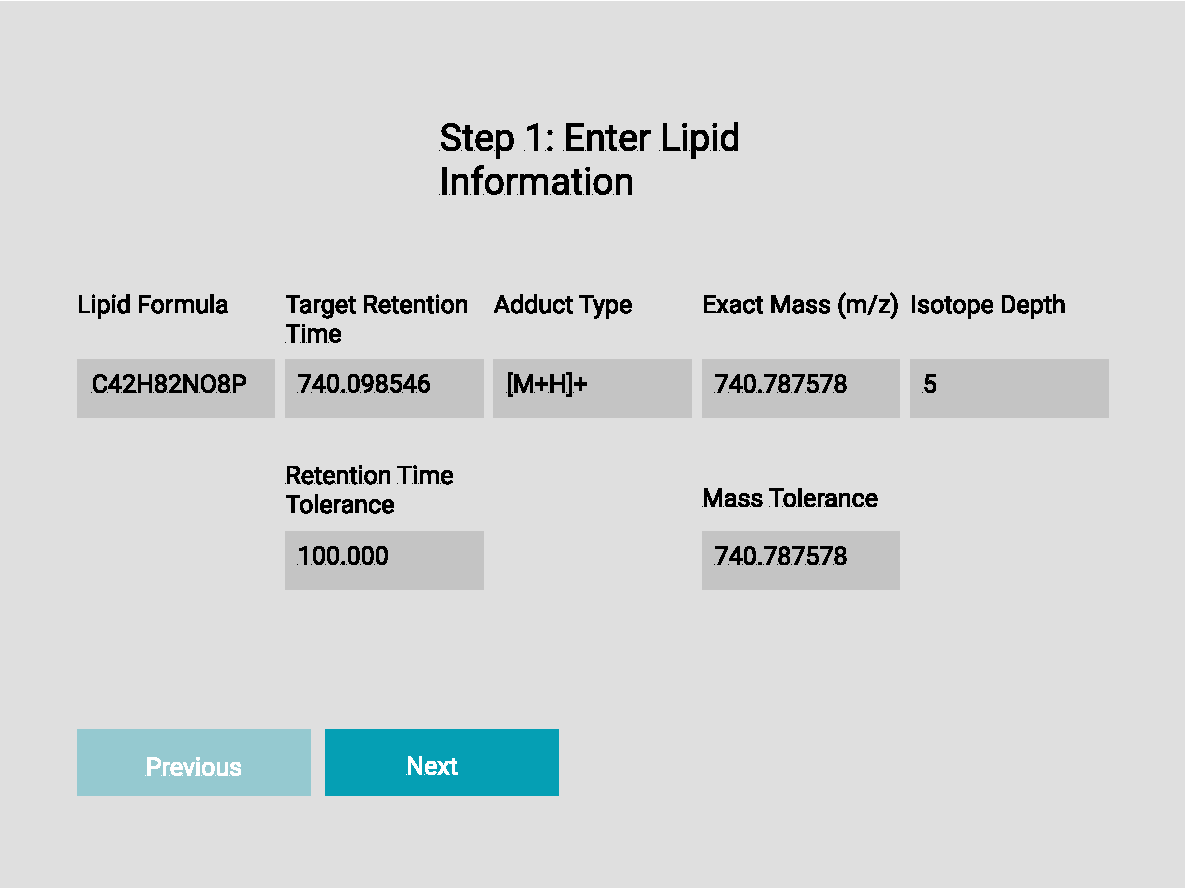
\includegraphics[width=\linewidth]{dissertation/images/wireframes/wireframe1.pdf}
        \caption{Lipid Details Screen}
    \end{subfigure}
    \begin{subfigure}{0.4\linewidth}
        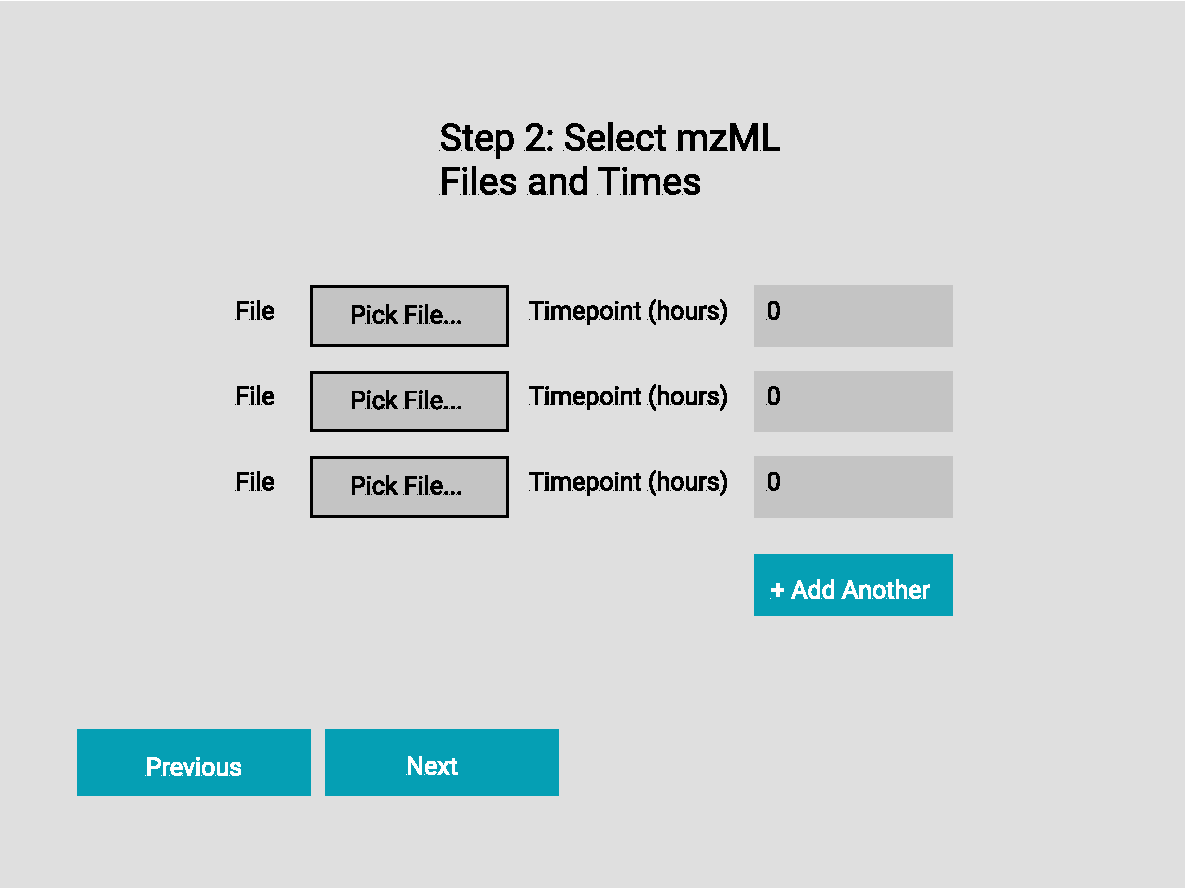
\includegraphics[width=\linewidth]{dissertation/images/wireframes/wireframe2.pdf}
    \caption{File Selection Screen}
    \end{subfigure}
    \begin{subfigure}{0.4\linewidth}
        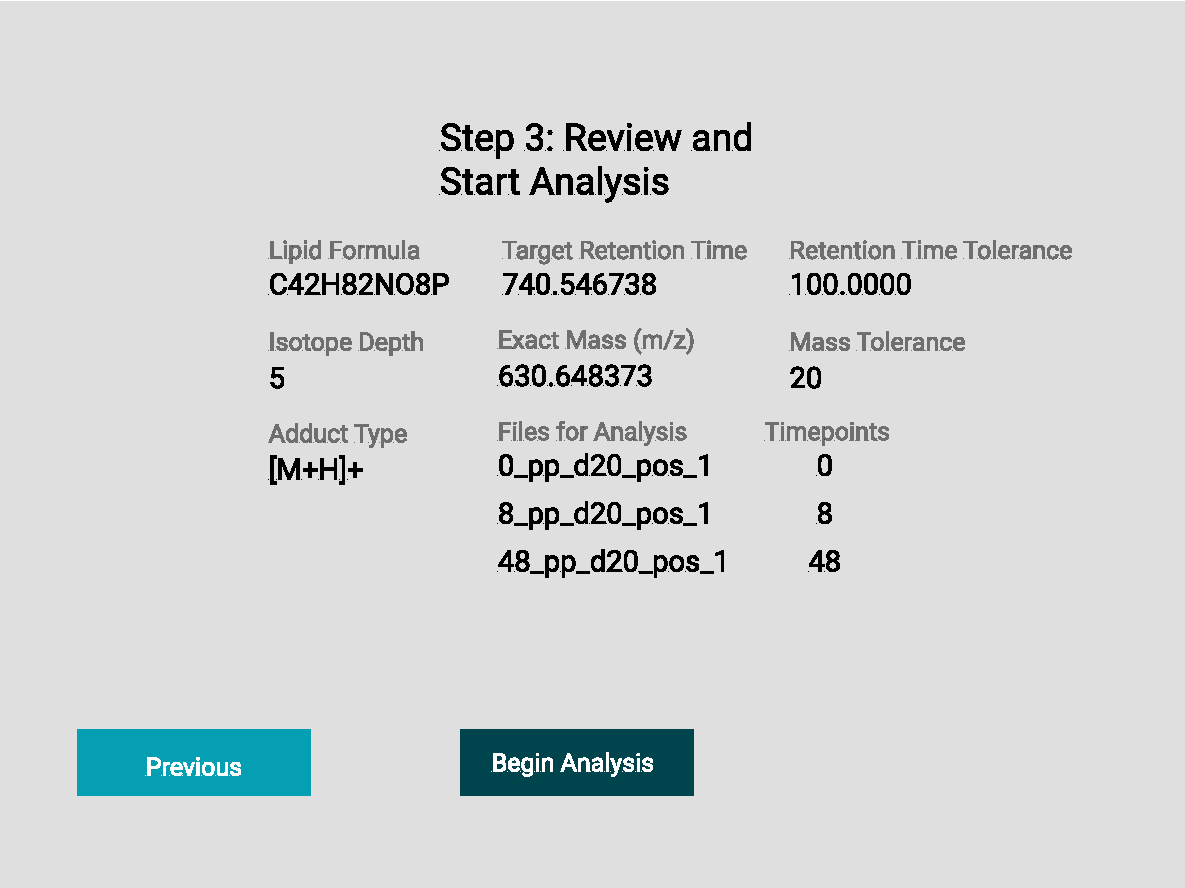
\includegraphics[width=\linewidth]{dissertation/images/wireframes/wireframe3.pdf}
    \caption{Input Summary Screen}
        \end{subfigure}
        \begin{subfigure}{0.4\linewidth}
        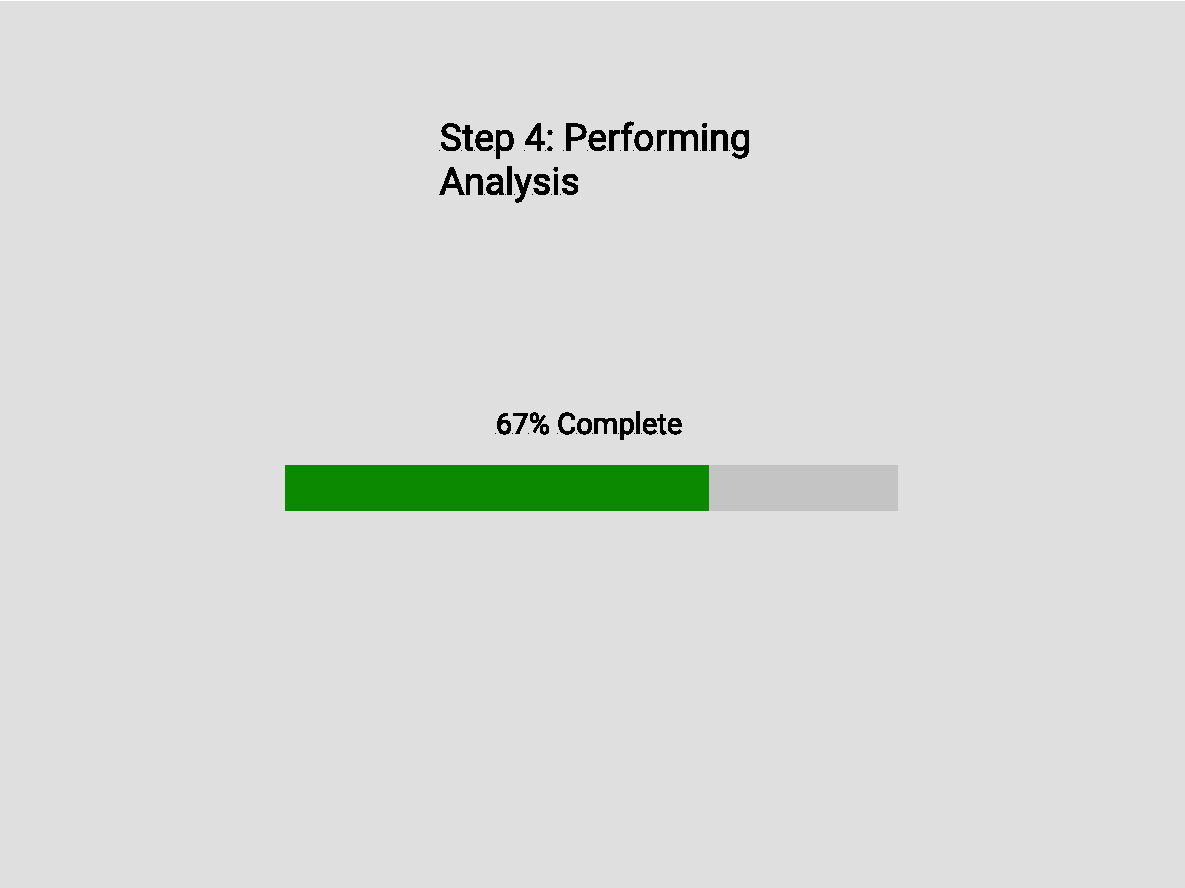
\includegraphics[width=\linewidth]{dissertation/images/wireframes/wireframe4.pdf}
    \caption{Analysis Progress Screen}
    \end{subfigure}
    \caption{The original wireframes for LiKInS. Each screen corresponds to one from the four-step design.}
    \label{fig:wireframes}
\end{figure}


Wireframes were not updated after the implementation of the original design. Instead, an agile approach was taken whereby any changes required would be made in-code on a feature branch before the next supervisor meeting. This allowed the developer to gain an understanding of PyQt (see section \ref{gui-implementation}) and how to create complex interfaces with it without wasting time creating further wireframes. Refinements were made to the UI throughout the project as usability problems arose.


\subsection{Four-step Design}
Based on the gathered requirements, it was clear that the user's journey through the application could be broken down into four distinct steps. While there were later deviations from this, with additional windows for defining new adducts as well as importing/exporting, the main user journey for performing analysis remained consistent throughout the development of LiKInS. The four steps, each of which maps to a screen within the application, were as follows:
\begin{enumerate}
    \item Lipid definition - At this stage, the user enters all information for all lipids they wish to define.
    \item File selection - The user chooses the MZML files they wish to analyse and enter the corresponding experiment timepoint for each file.
    \item Input summary - The user is given a chance to review all entered data and ensure it is correct before beginning analysis.
    \item Analysis progress - Analysis begins and the user is shown a progress bar denoting how much of the analysis has been performed as a percentage. Once analysis is completed, the user is shown the location of the output file on disk.
\end{enumerate}
Once implementation had begun, this design was modified slightly to fulfill additional requirements. The two features that required deviation was the implementation of importing/exporting groups of lipids and the definition of custom adducts. These features were designed around Windows platform conventions, with a standard file menu that can be accessed from any screen in the application. This would eventually include options for defining adducts, exporting lipids and importing lipids. When each of these options was clicked, a small modal window would be opened and the user would be prevented from interacting with the main window until it was closed. While this deviated from the existing \say{four-step design}, it allowed these new features to be seamlessly integrated with the existing system without a large-scale redesign.

\subsection{Information Required from the User}
It was clear from the onset that several pieces of information and files would be required from the user. Those that were initially believed to be necessary were as follows:
\begin{itemize}
    \item Lipid formula
    \item Target retention time
    \item Retention time tolerance(how far from the target retention should be searched for the peak intensity)
    \item Adduct type (defines how the target lipid is charged)
    \item Target mass (refers to m/z - the word \say{mass} is used due to poor understanding at this stage of development)
    \item Mass tolerance (\say{mass} refers to m/z and defines how far should be searched for peak)
\end{itemize}

Additionally, files to be analysed as well as the corresponding experiment time-point in hours would be required from the user.

Initially, the design only took into account the input of a single lipid. This was later updated to allow the input of a theoretically infinite number of lipids (with obvious technological limitations). It was also later established mass would not need to be manually entered as it could be calculated via the lipid formula and adduct.

\section{System Architecture} \label{system-architecture-design}
%Discuss GUI, state, lack of state management system being imposed by middleware. This gave flexibility but also required adherence to best practices.
Designing a robust system architecture was critical to ensuring the interactions between the user and the system would behave in an expected fashion. Since there was no database to speak of, standard state management and design patterns may not be the most optimal solution. The interactions between state and the interface are illustrated in \ref{fig:gui-state-interaction} It should be noted that the the following state management system was designed \textbf{after} the technology stack had been finalised.
\subsection{State Management System} \label{state-management-design}
Given the four-step nature of the application described in \ref{user-interface-design}, it was clear that traditional state management patterns were likely overkill. Each page of the application consists of basic components with no complicated interaction. A custom solution was designed, similar to the traditional Model-View-Controller architecture but without the intermediary Controller section. In essence, the view component would interact with the model component directly, via method calls. Each page would have its own state object and none of this logic would be shared except for the following caveats:
\begin{itemize}
    \item The input summary screen would need access to state from the lipid details screen.
    \item The input summary screen would need access to state from the file selection screen.
\end{itemize}

\begin{figure}[htb]
    \centering
    \includegraphics[scale=0.5]{dissertation/images/gui-state-diagram.pdf}
    \caption{Diagram showing the interaction design of screen and state objects. Each screen object accesses its respective state object via method calls and has no access to other state objects. State objects have no references to other classes.}
    \label{fig:gui-state-interaction}
\end{figure}

\section{Chapter Summary}
This chapter discussed the design of LiKInS including the user interface design with its four-step nature as well as an accompanying state management system to handle user interactions.


%==================================================================================================================================
\chapter{Implementation}
This chapter will discuss the implementation of LiKInS including the technology stack used, the GUI and state management implementations, packaging and finally testing.

\section{Technology Stack} \label{technology-stack}
There were several factors under consideration when deciding upon the programming language and libraries to be used. This section will discuss the technology choices that were considered and the rationale behind the final decision.
\subsection{Python}
Given that the prototype pipeline had already been implemented in Python, it was a clear candidate. It was already proven that powerful mass-spectrometry libraries existed and could be successfully implemented in Python as this had already been done. Using python would also allow for the reuse of code from the prototype pipeline, potentially allowing more time to be allocated to features beyond that of the analysis itself. Considering the key requirements in \ref{key-requirements} it was clear that, should Python be the final choice, we could run the application on Windows 10. It was also clear that any application created using Python could use an open-source license, as the language itself was open-source. The requirement of concern was the third: namely that by default, users would need to have Python properly installed along with all dependencies to be able to run it. This was deemed an unacceptable level of complexity and so a solution had to be found for this problem for Python to be a viable candidate.

To meet the final requirement, it was necessary to find a technology that can either:
\begin{itemize}
    \item  Compile Python code into a format that can be executed on Windows or;
\item Package the python runtime and all dependencies with the application so that it can be run in a single click by the user.
\end{itemize}
The best solution found was PyInstaller: a Python utility that gathers the current Python version along with all installed dependencies to produce a directory with all necessary files for the application to run. Within this directory is a file named "main.exe" which acts as an entrypoint to the application and so the entire application can be run in one click.


\subsection{Java}
The other primary contender was Java. Given that TOPPView is written in Java, it was clear that the libraries necessary to parse MZML files were already available in Java. Java also met all three of the key requirements: The application could run on Windows 10; anything developed with Java could be open-source; and the application could be compiled into a JAR file and run in one click, assuming the user has Java installed (this was viewed as acceptable as many other applications in this field, such as TOPPView, also require the installation of Java). Java also has the benefit of first-party GUI libraries such as Swing or JavaFX which are well supported and documented. The major downside to using java is of course that the code from the prototype pipeline would need to be completely rewritten.

\subsection{Final Choice}
In the end, Python was the final choice of language. This choice was mainly due to the fact that the prototype was already written in Python and so there was a large opportunity for reuse. Additionally, a Python application packaged with PyInstaller would be easier to run than the equivalent Java application as the user would not be required to have a JRE installed, although it is likely that the user wouldn't have any trouble installing a JRE.


\section{Graphical User Interface} \label{gui-implementation}
The final GUI was written in Python using PyQt5, a Python implementation of the popular Qt framework, developed by \cite{PyQt5}. This was chosen because it seemed to be the most feature rich and advanced Python GUI framework available and would allow for a look and feel that matches the parent operating system, providing a level of familiarity for users.

\begin{figure}[htb]
\centering
\begin{subfigure}{0.4\linewidth}
        \includegraphics[width=\linewidth]{dissertation/images/Screen1.png}
        \caption{Lipid Details Screen}
    \end{subfigure}
    \begin{subfigure}{0.4\linewidth}
        \includegraphics[width=\linewidth]{dissertation/images/screen2.png}
    \caption{File Selection Screen}
    \end{subfigure}
    \begin{subfigure}{0.4\linewidth}
        \includegraphics[width=\linewidth]{dissertation/images/Screen3.png}
    \caption{Input Summary Screen}
        \end{subfigure}
        \begin{subfigure}{0.4\linewidth}
        \includegraphics[width=\linewidth]{dissertation/images/Screen4.png}
    \caption{Analysis Progress Screen}
    \end{subfigure}
    \caption{The GUI screens for the final implementation. Two lipids are defined with 6 files. Each stage of the four-step process is shown.}
    \label{fig:gui-screens}
\end{figure}

All files related to UI components were placed in the \textbf{gui/} directory where each file generally represents a single screen, each of which may contain multiple classes. There is additionally a file named \say{custom\_components.py} which contains many classes, each of which extends a default Qt class. For example, as discussed in section \ref{usability-enhancements}, the default QSpinBox implementation provided a significant usability problem and so the scroll wheel functionality for these components had to be disabled. Instead of manually disabling them all, it was much easier to create a new component as a subclass of QSpinBox and disable the scrollwheel, then replace all QSpinBox objects with this new component.

A GUI controller class was written which simply acts as a wrapper around each of the four screens. Each of these screens were an attribute of this class and are instantiated within its constructor. This means that by instantiating the state controller, all GUI components are immediately instantiated. The state controller described in \ref{state-management-implementation} is also instantiated within the GUI controller.

The classes representing the four main screens(lipid details screen, file picker screen, input summary screen and progress screen) were connected to their respective state objects in the following way. The state object for that page, and only for that page, would be passed as an argument to the constructor of the GUI class. This would allow the GUI class to both read and write values to its state object. Since the GUI component generally only has access to its own state object and not those of other screens, we have a high separation of concerns between screens.

There are however exceptions to this model, generally pertaining to the input summary screen. This is due to this screen being used to display information from both the lipid details screen state and the file picker screen state. One option that was considered was to make copies of these state objects and provide these to the summary screen state to prevent it gaining access to the state of other screens however this was found to be cumbersome and could cause strange bugs, particularly when the copy of the state object was not up to date with the original as could be the case when information was changed. Instead, methods were defined within the state classes that would aggregate all data required by the summary screen and return a dictionary. Then, by passing these methods into the constructor of the state object for the summary screen, the summary screen only needed access to its own state object as with the other GUI classes. This allows us to provide the summary screen with access only to these aggregrator methods, allowing it to read up-to-date information without the possibility of accidentally adjusting something, maintaining our separation of concerns.

\section{State Management} \label{state-management-implementation}
Implementation of the state management system described in \ref{state-management-design} was carried out concurrently with the implementation of the GUI. Rather than implementing all user interface components then developing all state components, it was decided to implement a screen as described in \ref{user-interface-design} followed by the state component for that screen. This was helpful as it made it easy to stick strictly to the design of the state management system.

The class structure of the state management system directly mirrors that of the GUI with an overarching state controller class which has each screen state as an attribute. This is particularly useful as it means the state of any screen can be reset simply be creating a new state object for that screen. Likewise, the state of the entire application can be reset by creating a new state controller, as is done when the use clicks the restart button on the progress screen. As previously detailed, each state object has no access to outside classes(there are helper classes defined within the same file as some state object) and is encapsulated.

\section{Changes to Analysis Process}
There were several changes made to the analysis pipeline from prototype to final implementation in LiKInS. Firstly, most usages of mass-spec-utils were removed. In particular, the use of the adduct thesaurus which would download a .CSV file from a public GitHub containing calculation information for many adducts and this could then be used to calculate the mass of a lipid from its formula and adduct. With LiKInS, the user must enter this information manually however this provides a much greater level of flexibility as any lipids that are not already defined can simply be defined by the user.

Secondly, the entire process was split into two files: lipid\_kinetics.py and file\_creation.py. Methods were refactored to completely decouple the analysis process from the file creation process. This made it much easier to produce tests for each component individually.

Additionally, changes were made to allow the analysis process to be run on a separate thread, and to calculate how much data has been analysed. This was used to send update flags to the progress bar on the analysis progress screen. Code was also added to log progress, allowing for the implementation of a textual feedback console on the analysis progress screen.

In terms of performance, there was no optimisation from the prototype to the final implementation. This is because the performance of the prototype was already considered acceptable due to its large improvement over manually extracting data by-hand, the previous state of the art. It is however likely that the process could be greatly optimised in the future to minimize the parsing of each file. Currently, each file is parsed once per lipid and so a potential optimisation would be to parse each lipid once, gathering the data for every lipid as the file is parsed.

\section{Packaging}
The ease-of-use of the software was paramount for the target demographic and one key aspect of this is how easily the software can be installed and run. For Python to be a viable option, it was necessary to find a packaging solution to avoid making the user install Python themselves. This came in the form of PyInstaller, an open-source Python module that compiles Python source code into executable files for Windows, MacOS and Linux.

PyInstaller was found to be a good solution to this problem - when it worked. There were several points throughout the project when significant time was spent debugging PyInstaller issues. These issues were exacerbated as it would often compile the executable successfully, but the compiled executable would not run. While a console window would open, the Python error messages would be hard to read as they would refer to compiled versions of the source files with machine generated names.

As discussed in \ref{continuous-integration}, CI pipelines were set up for Windows, MacOS and Linux. While Windows was the only operating system mandated by requirements, having the software compiled for MacOS would make it more accessible for evaluation and for supervisor feedback as some contacts only had access to a Mac. This resulted in significant time being put into creating and maintaining a MacOS build pipeline with no test machine on which the software could be run. This eventually became unsustainable and so the MacOS pipeline was dropped and evaluation participants on Mac had to run the application with Python directly.

\subsection{One-file vs One-dir Modes}
PyInstaller offers two different modes: one-file mode and one-dir mode. On Windows, the one-file mode generates a single main.exe file and by running this file, all of the application files are unpacked into memory and are subsequently run. In contrast, one-dir mode generates a directory containing lots of compiled .dll files as well as a single main.exe file which acts as a entry-point to the application. The only real difference is that one-dir mode skips the unpacking step as files are always unpacked while one-file mode needs to go through this step and so startup time is significantly slower with one-file mode.

Initially, the packaging pipelines were set up using one-file mode. This would make it less confusing to run the software as there was just a single file included and the performance penalty at start-up was deemed to be acceptable. This became an issue when the addition of persistent files was implemented. All adducts, both default and custom, are stored using the positive.csv and negative.csv files. When a user defines a new adduct, a line is added to the appropriate file. This feature had a side-effect of breaking the one-file executable as the changes to the file would be removed each time the application was closed since persistent files were unpacked at run-time.

Two solutions were considered:
\begin{enumerate}
    \item Copy all persistent files to another location if there are not already copies there. Then, use these copies to store any persistent information, such as adducts.
    \item Use one-dir mode where these files are persistent and are not cleared when the application is exited.
\end{enumerate}
In retrospect, the first option would likely have been more elegant as it would keep the application as a single executable + persistent files while the latter was chosen as it was considerably less work to implement.

Had there been additional time for this project, a Windows install wizard would be a high priority feature. This would take the application, in one-directory form, and install it to a location of the users choosing. It would also place a shortcut in the users choice of the Windows desktop and/or start menu folder so they can use it without ever referring to its installation directory.


\section{Testing}\label{testing}
% Discuss creation of test files, justification behind what was/wasn't tested, any tests that were not present and perhaps should have been, difficulties in creating tests and final decision to use TOPPView
Unit testing is a major part of the development of robust software and the development of LiKInS presented several testing-related challenges that were somewhat unique to this type of development.

\subsection{GUI Testing}\label{gui-testing}
Early into the project, unit tests were written for the GUI. These tests mainly revolved around the moving of pages: if you click next, are you taken to the correct page? Since PyQt5 tests require the UI to be initialised, any testing machine would need display server capabilities to be able to run the tests and so these tests were not compatible with the continuous integration pipelines discussed in \ref{continuous-integration}. Additionally, the UI was prone to having its external behaviour altered often as new requirements were gathered and so these tests had to be rewritten on several occasions. After discussion with the project supervisor, it was decided that the return-on-investment of writing these tests was not worth it and so the decision was made to avoid further GUI unit tests.

\subsection{Testing the Analysis Pipeline}
Another significant complication came surrounding the writing of unit tests for the analysis process. Most of the analysis code was simply a refactored version of the prototype pipeline which did not come with unit tests. Given the complexity of the analysis process, it was difficult to determine whether or not the values from the functions and methods within the prototype were correct. The only real indicator of correctness was how the final curve looked in the output file. This presented an issue: how can we test a method or function when we don't know what a correct output value looks like? We could perform the analysis process manually, whereby a human goes through each file, manually extracts the values and determines the correct output as described in \ref{state-of-the-art} however this would have taken up a large amount of time, especially given that this process must be repeated each time a new unit test was written.

The final approach was simply to manually read values from TOPPview where it was feasible, which was the case for several methods, and where not feasible, simply trust the output values from the prototype pipeline. This would ensure that the final analysis process was at least as correct as the prototype and would still give the benefit of providing a safety net of unit tests without the writing of tests becoming a large burden on development speed.
\subsection{Test File Size}
The test files provided were up to 100MB in size. This meant that tests were relatively slow to run as these large files had to be at least partially parsed in each test. This was deemed unacceptable and so this issue needed to be addressed. The test files were cut down using an open-source application called MSConvert to only include scans that were relevant for the lipids defined within tests. This took file sizes down to between 1MB and 5MB and significantly increased the speed at which the test suite could run. It should be stressed that only scans that were not within the target mass and retention time ranges were cut out of these files and therefore the outcomes of tests were not changed by cutting the test files nor were the results invalidated. 

\subsection{Confidential Test Files}
The final issue surrounding test writing was due to the sensitive nature of test files. They were part of a separate research project being carried out by one of the clients and it was decided that these should not be publicly available until the research had concluded. This meant that test files could not be stored on the public GitHub repository and so a testing solution had to be engineered that would allow the writing and running of tests for the analysis process without making test files public.

This was done by making a number of changes to the way tests were structured. Firstly, tests were separated into two files: one for tests that depended on files and one for those that did not. Secondly, the continuous integration pipeline for Python tests was changed so as to only run tests that were not file-dependant. Finally, the file dependant tests were pointed to a directory outside of the repository where tests were located. In doing so, file dependant tests could still be run locally and no sensitive data was compromised.

Once these test files were deemed to no longer be sensitive, they were added to the repository and continuous integration was adjusted to run file-dependant tests.

\section{Chapter Summary}
The chapter discussed the implementation of LiKInS. This includes the technology stack used and why it was chosen, the GUI implementation alongside the accompanying state management system. It then went on to discuss changes that were made to the additional prototype pipeline, packaging and issues surrounding the writing of tests.



\chapter{Software Engineering Practices}
This chapter discusses software engineering practices and processes that were utilised during the development of LIKinS including version control, issue tracking, documentation, continuous integration and automated deployments. It also discusses the limited use of test-driven development in development and the limitations that were encountered in doing so.

\section{Version Control}
The repository was hosted on GitHub \citep{GitHub:online} which was chosen because it is generally the platform of choice for open-source projects and has all of the desired features including built-in issue tracking, a project wiki and continuous integration as well as a method of automated release. Each of these factors are discussed in this section.


\subsection{Feature Branching}
While this project was only worked on by a single developer, a branching strategy in conjunction with a continuous integration pipeline (see section \ref{continuous-integration}) was deemed to be essential in ensuring developer discipline throughout. The strategy used was \say{Feature Branching} as described by \cite{fowler_2020}. Essentially, a new branch was created for each feature, where a feature roughly corresponded to an issue in the issue tracker(see section \ref{issue-tracker}). Once each feature was complete, a pull request would be created and the pull request template would be filled in. Pull requests were used for two reasons, as opposed to merging directly: \begin{itemize}
    \item A pull request template could be used as a \say{checklist} by the developer to ensure that an issue was complete before merging onto the mainline branch.
    \item Continuous integration could be triggered on a pull request as a final safety net to ensure that the new branch passes tests and compiles correctly before a new feature was merged onto the mainline branch.
\end{itemize}
While this strategy was used for most features, there were occasions where a commit would be pushed straight to master but these were generally to change CI files and not changes to the application itself. In the latter stages of development, a release branch was added for deployment as described in \ref{deployment}.

\subsection{Pull Request Template}
A pull request template was used in the hopes of maintaining a level of developer discipline through this individual software project. Since nobody else would be contributing to the project, it was feared that slipping into bad practices and development habits could pose a serious issue towards the success of the project. The aforementioned template was designed to achieve the following goals:
\begin{itemize}
    \item Make the developer specify exactly how the PR solves the problem addressed by the feature branch.
    \item Make the developer list all work done in achieving the goal of the branch.
    \item Make the developer specify which issue is closed by the branch to automatically close it in the issue tracker.
    \item Make the developer fill out a checklist to ensure they have written appropriate tests and have no TODOs left for the issue in question.
\end{itemize}
Part of the pull request template is shown in figure \ref{fig:pr-template}.

\begin{figure}
    \centering
    \includegraphics[width=0.5\linewidth]{dissertation/images/PR-template.png}
    \caption{Part of a pull request that follows the pull request template as rendered on GitHub. }
    \label{fig:pr-template}
\end{figure}
\section{Issue Tracking}\label{issue-tracker}
GitHub's default issue tracker was a natural choice for keeping track of the project, with it one click away from the code repository itself. When a new requirement was gathered, it would first be converted into a user story, before being added to the issue tracker as one or more issues. Additionally, any bugs that were discovered would also be added as issues as well as any necessary documentation or CI updates.
\section{Documentation}
GitHub's inbuilt wiki feature was used to store and track design documents throughout the projects lifecycle. The most prominent of these was user stories: each story would be written out in the form \say{\textbf{As a} <user type> \textbf{I want to} <feature description> \textbf{So that} <justification for feature>} as requirements were gathered. Once it was time to start development on a batch of user stories, each one would be turned into one or more issues, which would then be put into the issue tracker. Upon completion of these user stories, they would have a strike-through put through them to denote them as complete. By storing stories separately from issues like this, it was easy to differentiate between immediately pressing issues and other user stories in the backlog whilst still keeping track of such issues.

\section{Continuous Integration \& Deployment} \label{continuous-integration} \label{deployment}
\begin{figure}[htb]
    \centering
    \scalebox{0.55}{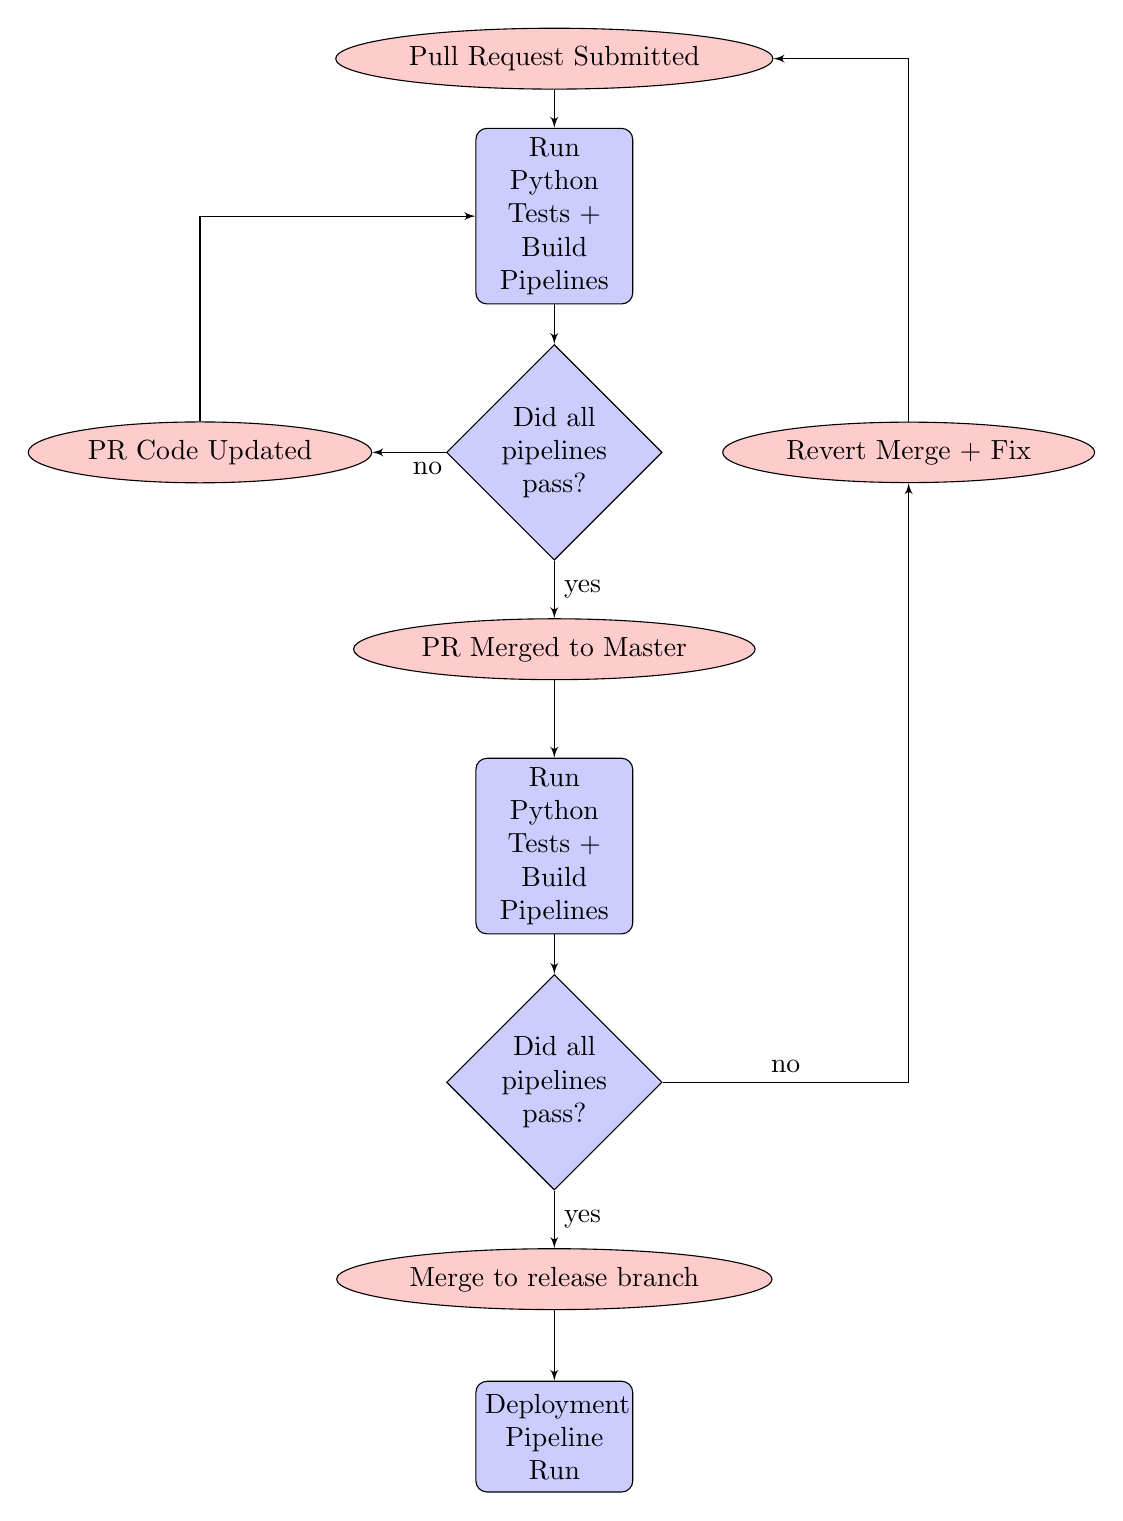
\begin{tikzpicture}[node distance = 2cm, auto]
    % Place nodes
    \node [cloud] (init) {Pull Request Submitted};
    \node [block, below of=init] (identify) {Run Python Tests + Build Pipelines};
    \node [decision, below of=identify] (decide) {Did all pipelines pass?};
    \node [cloud, left of=decide, node distance=4.5cm] (update) {PR Code Updated};
    \node [cloud, below of=decide, node distance=2.5cm] (merged) {PR Merged to Master};
    \node [block, below of=merged, node distance=2.5cm] (PR2) {Run Python Tests + Build Pipelines};
    \node [decision, below of=PR2, node distance=3cm] (decide2) {Did all pipelines pass?};
    \node [cloud, right of=decide, node distance=4.5cm] (revert) {Revert  Merge + Fix};
    \node [cloud, below of=decide2, node distance=2.5cm] (release) {Merge to release branch};
   \node [block, below of=release, node distance=2cm] (deploy) {Deployment Pipeline Run};
    % Draw edges
    \path [line] (init) -- (identify);
    \path [line] (identify) -- (decide);
    \path [line] (decide) -- node [near start] {no} (update);
    \path [line] (update) |- (identify);
    \path [line] (decide) -- node {yes}(merged);
    \path [line] (merged) -- (PR2);
    \path [line] (decide2) -| node [near start] {no} (revert);
    \path [line] (PR2) -- (decide2);
    \path [line] (revert) |- (init);
    \path [line] (decide2) -- node{yes}(release);
    \path [line] (release) -- (deploy);
\end{tikzpicture}}
    \caption{A flow-chart representing the feature acceptance process.}
    \label{fig:ci}
\end{figure}
One of the main reasons for using GitHub was the inclusion of free, easy to use continuous integration via GitHub Actions. Extensive use of this service was made for a variety of purposes. The following workflows were created:
\begin{enumerate}
    \item A pipeline to run all Python unit tests.
    \item A pipeline to build for Windows.
    \item A pipeline to build for MacOS.
    \item A pipeline to build for Linux.
    \item A pipeline to build for Windows and release compiled application. This acted as the main deployment mechanism.
\end{enumerate}
The overall acceptance procedure for a new pull request is illustrated in figure \ref{fig:ci}. Each of these will be discussed in turn.
\subsection{Testing Pipeline}
\cite{vasilescu} report that the use of automated testing within continuous integration results in 48\% more bugs being caught by development teams than without it and so using such automated testing appears to be an effective measure for identifying software defects. In the case of LiKInS, the testing pipeline was run upon each pull request to master and each push to master. This would run unit tests described in \ref{testing}, initially only running those that did not depend on test files until the content of  these files was no longer sensitive information.
 
 \subsection{Windows Build}
 The windows build pipeline was effective in ensuring that changes made to the application did not break the compilation process. There were numerous occasions where a change in codebase inadvertently broke the build process and this could be caught instantly as soon as the pull request was created and so could be remedied before being pushed to master.
 
 \subsection{MacOS and Linux Builds}
 While initially there was only a build pipeline for Windows, a counterpart for MacOS was soon created for the benefit of both the project supervisor and one of the clients, who were running MacOS machines.  A Linux pipeline was also created at this point as it was very little additional work and would serve the slim possibility of clients who were running Linux. As further changes were made, it became clear that the overhead to maintain all three build pipelines was rather large and without a machine to test the MacOS or Linux builds on, there was no way to test the built executable. Therefore, the decision was made to deprecate these builds. These pipelines would be run 
 
\subsection{Deployment}
GitHub includes a feature known as \say{GitHub Releases} which allows a built release of software to be stored separately from the repository itself and can be accessed by anybody whether they have a GitHub account or not. This seemed like the perfect way to distribute the application to evaluation participants. The final pipeline would once again build the Windows application but would then create a new release in GitHub releases with the built executable. This was done whenever there was a push to the release branch and so to create a new release one must simply merge master into the release branch.
'
\section{Test-Driven Development}
Test-Driven Development(TDD) is an agile methodology introduced in \say{Test-Driven Development By Example}\citep{kentbeck} which aims to produce inherently testable code alongside a suite of unit tests which both act as self-documentation(as tests essentially define the API for the piece of code being tested) and a safety net to provide instant feedback if a change has broken an existing piece of functionality.

With the clear benefits of TDD, it was decided from the outset that it would be an effective strategy for writing LiKInS in a robust and agile manner. It was especially suited due to the nature of the project: developer understanding of underlying processing was initially limited and requirements were likely to change often. Having a safety net of tests could help save time by identifying breaking changes early so they can be properly addressed.

Two main issues were encountered when attempting to implement TDD into the development process. Firstly, it was decided early that GUI tests would not be written as discussed in \ref{testing} therefore TDD was not used. Secondly, most of the analysis performing code was taken from the prototype so tests had to be written after-the-fact. While not TDD, efforts were still made to define the external behaviour of analysis code using tests. The benefits of this were realised later when some of this code was significantly refactored and its external behaviour could be proven to be the same.

Due to these issues, TDD was mostly used when writing state objects as well as functions surrounding persistent data storage and retrieval. Where it could be used, TDD was deemed to be an effective way to ensure software quality while still allowing agility with changing requirements.

\section{Chapter Summary}
This chapter discussed some of the software engineering and DevOps practices at play through the development of LiKInS. These include version control, issue tracking, documentation, continuous integration \& deployment and the use of test-driven development.

%==================================================================================================================================
\chapter{Usability Evaluation} \label{usability-evaluation}
This chapter discusses how the usability of the software was evaluated including the thinkaloud protocol, how gathered data was analysed, new functional requirements and reflections on the evaluation as a whole.


\section{Concurrent Think-aloud Protocol} \label{think-aloud-protocol}
%Introduce the thinkaloud protocol here, with reference tio Simon & Ericssons work
While several protocols for carrying out usability studies were considered, it soon became clear that any form of quantitative evaluation, such as the SUS scale or metrics on task time and number of errors, would not be suitable. This was because of the highly specialised nature of this piece of software: any potential participants would be required to have a certain level of knowledge surrounding the general analysis process as well as the surrounding jargon hence the number of potential participants was very small.

\section{Participants}
Four participants were recruited, each of whom were academics working in the field of metabolomics and so had the knowledge necessary to understand the underlying purpose of the software and related jargon. Three of these participants had previously seen the software in a much earlier state while one (participant 4) had not. This was during a meeting on the 3rd of November. Given the number of changes made since then, and the duration of time that had passed, learning effects from this demonstration were likely minimal.

\section{Evaluation Description}
The participant would join a video call with the evaluator. They would then be provided with two links: one led to the release page on GitHub while the other was a Google Drive folder containing two sets of reduced test files, one positive and one negative, as well as a spreadsheet detailing which lipids were contained in each set of files.

They would be given assistance in extracting both downloads and starting the software. Participants were then shown an example video, found on YouTube, of someone carrying out a think-aloud evaluation. This was done to give participants an example of the kind of commentary required to maximise the chances that each participant could provide useful insights into the usability of the software. At this point, the evaluation could begin.

Participants would be given a task to complete using the software and as they completed each task, they would verbalise their thoughts as much as possible. The evaluation was recorded using Microsoft Teams' inbuilt recording feature which would upload the recording to Microsoft Stream which would then generate a transcript. This transcript would then be downloaded and manually corrected. The final transcript would be processed as described in \ref{analysing-transcripts}.

There were four tasks in total, and they were as follows:
\begin{enumerate}
    \item \say{Perform analysis on three lipids from the positive data set.}
    \item \say{Define any three negative lipids and export them.}
    \item \say{Import the lipids from Task 2 and perform analysis on these lipids.}
    \item \say{Define a new positive adduct that is not in the list of positive adducts. An example of this would be [M+H-H20]. Define a lipid with the new adduct.}
\end{enumerate}
These four tasks were chosen as together they would allow each participant to interact with every UI element of the software, including those contained within the file menu.

\section{Analysing Transcripts} \label{analysing-transcripts}
A rudimentary selective coding technique was used to analyse the transcripts in order to identify changes that would improve the usability of the application. Statements of interest would be highlighted to show the key idea being proposed. These key ideas were then categorised and could be matched across the four participants in order to identify which aspects of the system were difficult to use for participants. 

For example, one of the categories was \say{ambiguous label}. This was used when a participant expressed that they did not understand the meaning of a field label. Two out of four participants expressed that they did not know what was meant by \say{Isotope depth} and so it was clear that this label presented a usability problem that needed to be addressed.

\begin{figure}[htb]
    \begin{subfigure}{0.5\textwidth}
        \centering
        \includegraphics[width=\textwidth]{dissertation/images/transcript_page_1.png}    
        \label{fig:final} 
    \end{subfigure}
        \begin{subfigure}{0.5\textwidth}
        \centering
        \includegraphics[width=\textwidth]{dissertation/images/transcript_page_2.png}    
        
        \label{fig:final} 
    \end{subfigure}
    \caption{An excerpt from one of the evaluation transcripts. Text is annotated using colour and a legend is included denoting the meaning of each colour.}
\end{figure}

\section{Results}
Upon analysis of the transcripts, the following issue categories were identified:
\begin{itemize}
    \item Ambiguous Label - Participant expressed that they did not understand the meaning of a label or the lack of a label altogether.
    \item Desired Feature - Participant expressed that they would like a feature that does not currently exist within the software.
    \item Input Error - Participant entered an incorrect value or accidentally changed a correct value.
    \item Confusion - Participant expressed a general confusion as to what to do next.
\end{itemize}

\subsection{Ambiguous Label}
Several labels were identified as being ambiguous:
\begin{itemize}
    \item Two participants expressed that they did not understand the meaning of \say{Isotope Depth}.
    \item One participants noted the lack of a label for the file extension of exported files on the export screen.
    \item Two participants expressed confusion at the meaning of \say{name} labels(one for adduct name and one for lipid name) not realising that the values entered would not affect the results of the analysis process.
    \item Three participants expressed confusion as to the meaning of \say{time} when choosing files although all eventually realised the true meaning.
    \item One participant did not understand the meaning of \say{multiplication value} within the adduct definition form.
    \item One participant desired additional \say{guides} to provide more information as to the meaning of certain fields. 
\end{itemize}
\subsection{Desired Feature}
The following features were requested:
\begin{itemize}
    \item One participant wanted to \say{carry over information from lipid to lipid} so that common attributes can be specified once and would be set for all lipids.
    \item One participant wanted to save the files from a previous run(much like lipid exporting) to avoid having to re-enter upon a later run.
    \item One participant suggested additional default adducts for the future, this was prior to realising they can define their own.
    \item One participant suggested that they preferred to work in minutes instead of seconds for retention time.
\end{itemize}
\subsection{Input Error}
The use of spinbox widgets for entering numerical values presented an obvious usability problem. One participant accidentally changed the value of a spinbox on 10 separate occasions, while another did so on 4 occasions. This was because the mouse wheel adjusts the value of a spinbox, so as the participant scrolled up and down, they accidentally changed values. The participants that did not make this error opted to scroll by dragging the sidebar instead of using the mouse wheel.
\subsection{Confusion}
This category is more general and denotes occasions where participants got stuck or expressed uncertainty and where these occasions do not fit into any other category.
\begin{itemize}
    \item One participant expressed confusion as to the functionality of the \say{Add Lipid} button, believing it would submit previously entered data when it actually initialised a new form to add a new lipid.
    \item Two participants got stuck when trying to find the export menu, not realising that the file menu existed.
    \item There were several other items of confusion that were not directly related to the software. These were mainly due to the instructions given to participants or a misunderstanding of those instructions.
\end{itemize}

\section{Usability Enhancements} \label{usability-enhancements}

It was decided that the following enhancements would be made based on the evaluation results:
\begin{itemize}
    \item The following labels would be altered:
    \begin{itemize}
        \item \say{Isotope Depth} would be changed to \say{Number of Isotopes}.
        \item Time units would be added to the time labels within the file picker screen.
        \item \say{Add Lipid} would become \say{New Lipid}.
        \item \say{Add files} would become \say{Choose Files}    
        \item JSON file extension would be added after file name in export form.
    \end{itemize}
    \item Tooltips explaining the meaning of a term were added to the following UI elements:
    \begin{itemize}
        \item Lipid Name.
        \item Isotope Depth.
        \item Adduct addition value.
        \item Adduct multiplication value.
    \end{itemize}
    \item When adding a new lipid, the view for all previous lipids would automatically be collapsed.
    \item The default spinbox implementation was extended to prevent the mouse wheel from changing the value of spinboxes.
    \item Adduct nickname was removed from the application.
\end{itemize}

\section{Reflections}
\subsection{Confounding Factors}
There were several factors that could not be controlled for between participants. Since evaluations had to be done remotely, each participant used their own computer and monitor. This could lead to the software appearing slightly differently for each participant. Similarly, participant 1 did not have access to a Windows machine and so had to carry out the evaluation on a machine running MacOS Mojave. 

\subsection{Software Bugs}\label{bugs}
There were several bugs encountered during each of the evaluations which caused some tasks to be cut short. Were it not for time constraints, it would have been more far more desirable to carry out evaluations after more thorough testing to ensure that participants could fully complete each task as this could lead to further insights into the usability of the software.

\section{Chapter Summary}
This chapter discussed the usability evaluation of the software. This encompasses: the protocol used; the recruitment of participants; how the evaluation was carried out; how the data was analysed; the final results; new usability requirements gathered from the results; and reflections on the evaluation as a whole.


%==================================================================================================================================
\chapter{Conclusion}
This chapter summarises this dissertation before discussing developer reflections on the project as a whole. It then goes on to discuss potential future development of LiKInS.
\section{Summary}
This dissertation discussed the design and development of LiKInS(Lipid Kinetics Inference Software) from gathering requirements through to evaluating usability. Mass-spectrometers are used to measure the products of isotope labelling experiments and prior to the development of LiKInS, there was not publicly available software for inferring lipid kinetics over time. LiKInS was developed with the assistance of clients from the University of the Highlands and Islands and Glasgow Polyomics and aimed to automate a manual process previously undertaken by one of these clients for their PhD.

The previous state of the art for this process was a human manually going through each file and extracting values by hand. This is a labour intensive and highly error prone process with a time complexity of $O(lmn)$ for $l$ lipids with $m$ isotopes being analysed and $n$ data files. While this is within polynomial time and is trivial for a computer to perform, it is incredibly time consuming for a human. LiKInS was written in Python and leveraged a prototype, also written in Python, as the basis for the underlying analysis.

Before development could begin, the complex problem needed to be understood by the sole developer. This was done through manual reading of prototype code, the reading of an academic paper provided by the project supervisor and the reviewing of recorded explanations from supervisor meetings. Further clarifications could then be made in subsequent supervisor meetings. Requirements were initially gathered as user stories before being converted into one or more actionable issues with appropriate labels.

The user interface design contained four screens: one for defining lipids; one for choosing files and entering their corresponding experiment time points; one for reviewing all entered data; and one to view the progress of the analysis pipeline. A corresponding custom state management system was devised with one state object for each of these screens. 

The application was written using a technology stack centered around Python with the graphical user interface being written in PyQt5. State was managed using the custom state management system with a one-to-one relationship between state objects and GUI objects. There were several testing related challenges throughout development that needed to be addressed. User interface testing was seen to provide little value for the amount of effort required to write them and so it was decided that these tests should not be written. Since test files were considered as sensitive information, workarounds had to be found to avoid storing this data in a public GitHub repository until it was no longer considered sensitive.

Many software engineering and DevOps practices were utilised in the development of LiKInS. Version control was done via Git with the repository being hosted on GitHub. Feature branching was used to maintain developer discipline throughout the project. Other GitHub features were used to assist in the project: GitHub's issue tracker was used to manage the product backlog; GitHub's \say{wiki} feature was used to manage project documentation; GitHub actions was used to run continuous integration pipelines; and GitHub releases was used to deploy the application. Test-driven development was utilised to ensure code quality and to catch newly introduced bugs however the nature of development made TDD difficult in some cases and so its use was somewhat limited.

With usability being of primary concern, a usability evaluation was carried out with LiKInS to identify areas of the implementation that were difficult to use. The concurrent think-aloud protocol was used where participants completed a series of tasks provided by the evaluate and verbalised their thoughts whilst completing each task. Transcripts were taken and phrases were then categorised into one of four categories, allowing areas of common difficulty to be identified, quantified and addressed. Many labels were found to be ambiguous or difficult to understand and users expressed great confusion as to the location of exported files.


\section{Reflections}
There are many aspects of development that, if this project were to be repeated, would be done differently whilst others would remain largely the same. Reflections that yield potentially valuable insights are listed below.

\subsection{Requirements Gathering}
Given the specialised nature of the application at hand, gathering accurate requirements was crucial and the methods used were found to be effective in ensuring requirements were captured with no major issues arising from misinterpreted requirements. The recording and reviewing of meetings was a large part of this success as it allowed misunderstood areas to be noted and then addressed at subsequent meetings. Likewise, the manual inspection of prototype code allowed phenomena described in meetings to be linked to their implementation. Whilst there was significant time and effort put into understanding these requirements, this would likely always be the case with such a specialist application.

\subsection{Design}
Overall, the design stage was successful in that the final implementation largely reflected the initial design with refinements being made throughout as one would expect. One aspect of design that could have avoided errors later on is to do with wireframes: new requirements mandated the creation of screens that were not part of the initial four-step design (file import/export) and so these new screens did not have wireframes prior to implementation. Had these screens been at least partially designed, feedback could have been gathered from clients and some usability issues could perhaps have been avoided. More generally, more constant client contact could have avoided some issues throughout the project however, given that clients were not required to give up their time in any way, the decision was made not to ask for too much feedback.

\subsection{Implementation}
% As with any software project, issues arose throughout the implementation of LiKInS. These will be discussed in turn.
\subsubsection{Technology Stack}
If this project was to be repeated, the Python stack described in section \ref{technology-stack} would likely be swapped with the proposed Java stack for the following reasons:
\begin{itemize}
    \item PyInstaller was found to be cumbersome and difficult to work with. Large amounts of time were spent debugging and fixing issues with it not detecting certain dependencies. Changes to the codebase would commonly require updating PyInstaller's configuration and it generally took more time than it should have. Compiling a Java application into a JAR file would likely have been much less of a problem and is still of minimal inconvenience to the end-user.
    \item The choice of GUI library on Python, PyQt5, was very poorly documented and was found to be lacking in certain functionality and base components. For example, the included layout components were very basic and did not include any dynamic layouts, such as collapsible accordion views, which had to be implemented by hand. Contrasting this with the mature JavaFX which includes an accordion component by default and is documented with standard, complete javadocs and it becomes clear that Java likely would have been a better choice resulting in a more pleasing GUI.
    \item As is mentioned in \ref{testing}, GUI tests were quickly abandoned when it became clear that the effort to reward ratio for PyQt5 tests was very high and that it would be impossible to run them on CI with no window manager. JavaFX supports GUI testing without requiring the GUI to be instantiated. This would allow such GUI tests to be quickly written and included in CI.
\end{itemize}

\subsubsection{State Management}
The chosen state management system was found to be very effective and is one of the highlights of this project given that it did not require any significant redesign during implementation and was instead flexible enough to handle all new requirements without being overly complex. It is however true that if the previously described technology changes were made, platform conventions may well impose a different state management system.

\subsubsection{Testing}
Whilst the written test suite was effective and did assist in catching breaking changes, the decision to drop user interface tests had a negative impact on the robustness of the final product and would possibly have assisted in catching bugs earlier. Several bugs were introduced upon the implementation of lipid importing that were only caught during evaluation and which a comprehensive test suite would likely have caught early. This does not however change the fact that, under the circumstances, foregoing user interface tests was justified under the circumstances given the reasoning provided in section \ref{gui-testing}.

\subsection{Version Control}
\subsubsection{Feature Branching}
While some would argue that no branching strategy is necessary in a project with a sole developer, feature branching was found to be an effective tactic in ensuring developer discipline and repository organisation. This kept each commit focused on the issue related to its branch and prevented deviation from whichever task was currently being completed. There were occasionally very small changes that were pushed directly to the master branch and the branching strategy did not interfere with the ability to perform these changes when required.

\subsubsection{Pull Request Template}
The pull request template was successful in its stated goals, ensuring that the requirements of each issue were fully met before the corresponding branch could be pulled into master.

\subsection{Continuous Integration}
While this is no surprise, the use of continuous integration throughout the project undoubtedly saved time. There were several occasions when bugs or problems building new changes were only highlighted upon the running of testing and build pipelines after a pull request. Without such safeguards, these issues would have been caught later and would be more difficult to fix.

\subsection{Usability Evaluation}
As discussed in section \ref{usability-evaluation}, the evaluation methods available were somewhat restricted due to the small number of potential participants. This issue was unavoidable and the best solution was chosen under the circumstances. The results were perhaps affected by a number of bugs that were found during evaluations and additional testing and checks could potentially have caught these. Additionally, a further round of usability testing could have verified that the changes made did in fact improve usability however participants would have now been familiar with the software and learning effects would have significantly biased results in favour of increased usability.


\section{Future Developments}

\subsection{Additional Features}
If one were to continue development of LiKInS, there are several avenues they may wish to pursue beyond further usability enhancements. Firstly, there are the original stretch goals of this project that were not fulfilled.

\subsubsection{Re-analysis of Single Values} Should the output produce a value that appears to be an error(e.g. nothing was found within target ranges or value does not follow the expected pattern), the user should be able to somehow select that value, adjust analysis parameters and run analysis on only the designated area.
\subsubsection{In-app Visualisations}Make data visualisations visible and interactive within the application itself instead of automatically opening the output file. This would be a simple quality-of-life improvement. 


While those are the original stretch goals for the project, there are additional improvements that could be made:

    \subsubsection{Error reporting.} The application could have checks in place to see if a potential error was made in the analysis(or within an input file). These errors could be reported within the console on the progress screen and optionally saved to log files.
    \subsubsection{In-place Error Reporting} This would build further upon error reporting by pausing analysis when a potential error has occurred and offering the user the option to tweak parameters and run that value again or to simply continue.
   \subsubsection{Expanded exporting.} Exporting could be expanded to allow the exporting of analysis file locations and corresponding experiment time-points. This would allow researchers to easily run a full analysis again without the need to re-enter files and time-points.

\subsection{Performance Enhancements}
As is discussed in \ref{key-requirements}, the speed of analysis was not an important factor in the development of LiKInS and as such, the original analysis process from the prototype pipeline was largely unchanged. It would almost certainly be possible in the future to optimize this process to reduce the amount of file parsing involved, hence reducing analysis times.

%==================================================================================================================================
%
% 
%==================================================================================================================================
%  APPENDICES  

\begin{appendices}

\chapter{Appendices}



\end{appendices}

%==================================================================================================================================
%   BIBLIOGRAPHY   

% The bibliography style is abbrvnat
% The bibliography always appears last, after the appendices.

\bibliographystyle{abbrvnat}

\bibliography{l4proj}

\end{document}
